% GNUPLOT: LaTeX picture with Postscript
\begingroup
  \makeatletter
  \providecommand\color[2][]{%
    \GenericError{(gnuplot) \space\space\space\@spaces}{%
      Package color not loaded in conjunction with
      terminal option `colourtext'%
    }{See the gnuplot documentation for explanation.%
    }{Either use 'blacktext' in gnuplot or load the package
      color.sty in LaTeX.}%
    \renewcommand\color[2][]{}%
  }%
  \providecommand\includegraphics[2][]{%
    \GenericError{(gnuplot) \space\space\space\@spaces}{%
      Package graphicx or graphics not loaded%
    }{See the gnuplot documentation for explanation.%
    }{The gnuplot epslatex terminal needs graphicx.sty or graphics.sty.}%
    \renewcommand\includegraphics[2][]{}%
  }%
  \providecommand\rotatebox[2]{#2}%
  \@ifundefined{ifGPcolor}{%
    \newif\ifGPcolor
    \GPcolortrue
  }{}%
  \@ifundefined{ifGPblacktext}{%
    \newif\ifGPblacktext
    \GPblacktexttrue
  }{}%
  % define a \g@addto@macro without @ in the name:
  \let\gplgaddtomacro\g@addto@macro
  % define empty templates for all commands taking text:
  \gdef\gplbacktext{}%
  \gdef\gplfronttext{}%
  \makeatother
  \ifGPblacktext
    % no textcolor at all
    \def\colorrgb#1{}%
    \def\colorgray#1{}%
  \else
    % gray or color?
    \ifGPcolor
      \def\colorrgb#1{\color[rgb]{#1}}%
      \def\colorgray#1{\color[gray]{#1}}%
      \expandafter\def\csname LTw\endcsname{\color{white}}%
      \expandafter\def\csname LTb\endcsname{\color{black}}%
      \expandafter\def\csname LTa\endcsname{\color{black}}%
      \expandafter\def\csname LT0\endcsname{\color[rgb]{1,0,0}}%
      \expandafter\def\csname LT1\endcsname{\color[rgb]{0,1,0}}%
      \expandafter\def\csname LT2\endcsname{\color[rgb]{0,0,1}}%
      \expandafter\def\csname LT3\endcsname{\color[rgb]{1,0,1}}%
      \expandafter\def\csname LT4\endcsname{\color[rgb]{0,1,1}}%
      \expandafter\def\csname LT5\endcsname{\color[rgb]{1,1,0}}%
      \expandafter\def\csname LT6\endcsname{\color[rgb]{0,0,0}}%
      \expandafter\def\csname LT7\endcsname{\color[rgb]{1,0.3,0}}%
      \expandafter\def\csname LT8\endcsname{\color[rgb]{0.5,0.5,0.5}}%
    \else
      % gray
      \def\colorrgb#1{\color{black}}%
      \def\colorgray#1{\color[gray]{#1}}%
      \expandafter\def\csname LTw\endcsname{\color{white}}%
      \expandafter\def\csname LTb\endcsname{\color{black}}%
      \expandafter\def\csname LTa\endcsname{\color{black}}%
      \expandafter\def\csname LT0\endcsname{\color{black}}%
      \expandafter\def\csname LT1\endcsname{\color{black}}%
      \expandafter\def\csname LT2\endcsname{\color{black}}%
      \expandafter\def\csname LT3\endcsname{\color{black}}%
      \expandafter\def\csname LT4\endcsname{\color{black}}%
      \expandafter\def\csname LT5\endcsname{\color{black}}%
      \expandafter\def\csname LT6\endcsname{\color{black}}%
      \expandafter\def\csname LT7\endcsname{\color{black}}%
      \expandafter\def\csname LT8\endcsname{\color{black}}%
    \fi
  \fi
    \setlength{\unitlength}{0.0500bp}%
    \ifx\gptboxheight\undefined%
      \newlength{\gptboxheight}%
      \newlength{\gptboxwidth}%
      \newsavebox{\gptboxtext}%
    \fi%
    \setlength{\fboxrule}{0.5pt}%
    \setlength{\fboxsep}{1pt}%
\begin{picture}(7200.00,3600.00)%
    \gplgaddtomacro\gplbacktext{%
      \csname LTb\endcsname%%
      \put(618,750){\makebox(0,0)[r]{\strut{}1}}%
      \csname LTb\endcsname%%
      \put(618,1170){\makebox(0,0)[r]{\strut{}1.02}}%
      \csname LTb\endcsname%%
      \put(618,1590){\makebox(0,0)[r]{\strut{}1.04}}%
      \csname LTb\endcsname%%
      \put(720,354){\makebox(0,0){\strut{}0}}%
      \csname LTb\endcsname%%
      \put(1363,354){\makebox(0,0){\strut{}0.125}}%
      \csname LTb\endcsname%%
      \put(2006,354){\makebox(0,0){\strut{}0.25}}%
      \csname LTb\endcsname%%
      \put(2648,354){\makebox(0,0){\strut{}0.375}}%
      \csname LTb\endcsname%%
      \put(3291,354){\makebox(0,0){\strut{}0.5}}%
      \csname LTb\endcsname%%
      \put(3934,354){\makebox(0,0){\strut{}0.625}}%
      \csname LTb\endcsname%%
      \put(4577,354){\makebox(0,0){\strut{}0.75}}%
      \csname LTb\endcsname%%
      \put(5220,354){\makebox(0,0){\strut{}0.875}}%
      \csname LTb\endcsname%%
      \put(5862,354){\makebox(0,0){\strut{}1}}%
      \csname LTb\endcsname%%
      \put(6505,354){\makebox(0,0){\strut{}1.125}}%
      \csname LTb\endcsname%%
      \put(7148,354){\makebox(0,0){\strut{}1.25}}%
    }%
    \gplgaddtomacro\gplfronttext{%
      \csname LTb\endcsname%%
      \put(24,1170){\rotatebox{-270}{\makebox(0,0){\strut{}$1\sigma$ histogram}}}%
      \csname LTb\endcsname%%
      \put(3934,75){\makebox(0,0){\strut{}Energy (GeV)}}%
    }%
    \gplgaddtomacro\gplbacktext{%
      \csname LTb\endcsname%%
      \put(618,1800){\makebox(0,0)[r]{\strut{}0}}%
      \csname LTb\endcsname%%
      \put(618,2227){\makebox(0,0)[r]{\strut{}50}}%
      \csname LTb\endcsname%%
      \put(618,2653){\makebox(0,0)[r]{\strut{}100}}%
      \csname LTb\endcsname%%
      \put(618,3080){\makebox(0,0)[r]{\strut{}150}}%
      \csname LTb\endcsname%%
      \put(618,3506){\makebox(0,0)[r]{\strut{}200}}%
      \csname LTb\endcsname%%
      \put(720,1614){\makebox(0,0){\strut{}}}%
      \csname LTb\endcsname%%
      \put(1363,1614){\makebox(0,0){\strut{}}}%
      \csname LTb\endcsname%%
      \put(2006,1614){\makebox(0,0){\strut{}}}%
      \csname LTb\endcsname%%
      \put(2648,1614){\makebox(0,0){\strut{}}}%
      \csname LTb\endcsname%%
      \put(3291,1614){\makebox(0,0){\strut{}}}%
      \csname LTb\endcsname%%
      \put(3934,1614){\makebox(0,0){\strut{}}}%
      \csname LTb\endcsname%%
      \put(4577,1614){\makebox(0,0){\strut{}}}%
      \csname LTb\endcsname%%
      \put(5220,1614){\makebox(0,0){\strut{}}}%
      \csname LTb\endcsname%%
      \put(5862,1614){\makebox(0,0){\strut{}}}%
      \csname LTb\endcsname%%
      \put(6505,1614){\makebox(0,0){\strut{}}}%
      \csname LTb\endcsname%%
      \put(7148,1614){\makebox(0,0){\strut{}}}%
    }%
    \gplgaddtomacro\gplfronttext{%
      \csname LTb\endcsname%%
      \put(126,2653){\rotatebox{-270}{\makebox(0,0){\strut{}Events}}}%
      \csname LTb\endcsname%%
      \put(3934,1558){\makebox(0,0){\strut{}}}%
      \csname LTb\endcsname%%
      \put(6009,2409){\makebox(0,0)[l]{\strut{}No syst}}%
      \csname LTb\endcsname%%
      \put(6309,2595){\makebox(0,0)[l]{\strut{}1\%}}%
      \csname LTb\endcsname%%
      \put(6309,2781){\makebox(0,0)[l]{\strut{}2\%}}%
      \csname LTb\endcsname%%
      \put(6309,2967){\makebox(0,0)[l]{\strut{}3\%}}%
      \csname LTb\endcsname%%
      \put(6309,3153){\makebox(0,0)[l]{\strut{}4\%}}%
      \csname LTb\endcsname%%
      \put(6309,3339){\makebox(0,0)[l]{\strut{}5\%}}%
    }%
    \gplbacktext
    \put(0,0){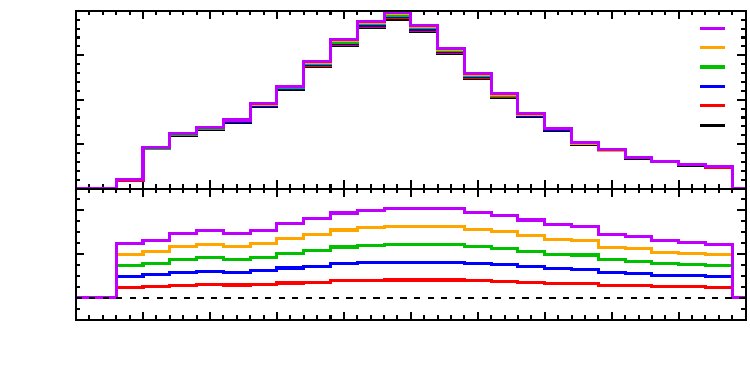
\includegraphics{nuenorm_E_RHC_sys1}}%
    \gplfronttext
  \end{picture}%
\endgroup
